\section{Kiến trúc mô hình ViHealthBERT}
\subsection{Transformer và BERT}
Mô hình Transformer ứng dụng cơ chế self-attention và multi-head attention được giới thiệu lần đầu trong paper Attention is All You Need\cite{DBLP:journals/corr/VaswaniSPUJGKP17}. 
\begin{figure}
\centering
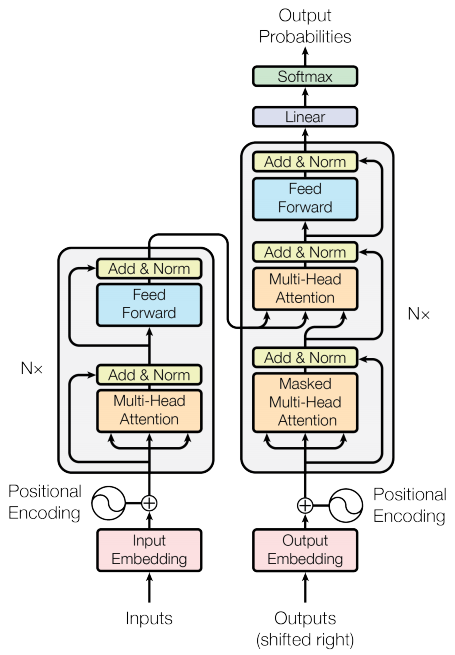
\includegraphics[scale=.35]{img/transformer.png}
\caption{Kiến trúc Transformer\cite{DBLP:journals/corr/VaswaniSPUJGKP17}}
\label{fig:transformer_diagram}
\end{figure}
Phần Encoder của Transformer được sử dụng trong mô hình BERT (\textbf{B}idirectional \textbf{E}ncoder \textbf{R}epresentations from \textbf{T}ransformers)\cite{devlin-etal-2019-bert}. Trong bài báo, BERT được giới thiệu có 2 phiên bản với các siêu tham số (hyperparameters) và số lượng tham số huấn luyện (training parameters) khác nhau:
\begin{itemize}
\item \textbf{BERT\textsubscript{base}}: 12 Transformer encoder layers, 768 hidden units, 12 attention heads, 110 triệu parameters.
\item \textbf{BERT\textsubscript{large}}: 24 Transformer encoder layers, 1024 hidden units, 16 attention heads và 340 triệu parameters.
\end{itemize}
\begin{figure}
\centering
\resizebox{\textwidth}{!}
{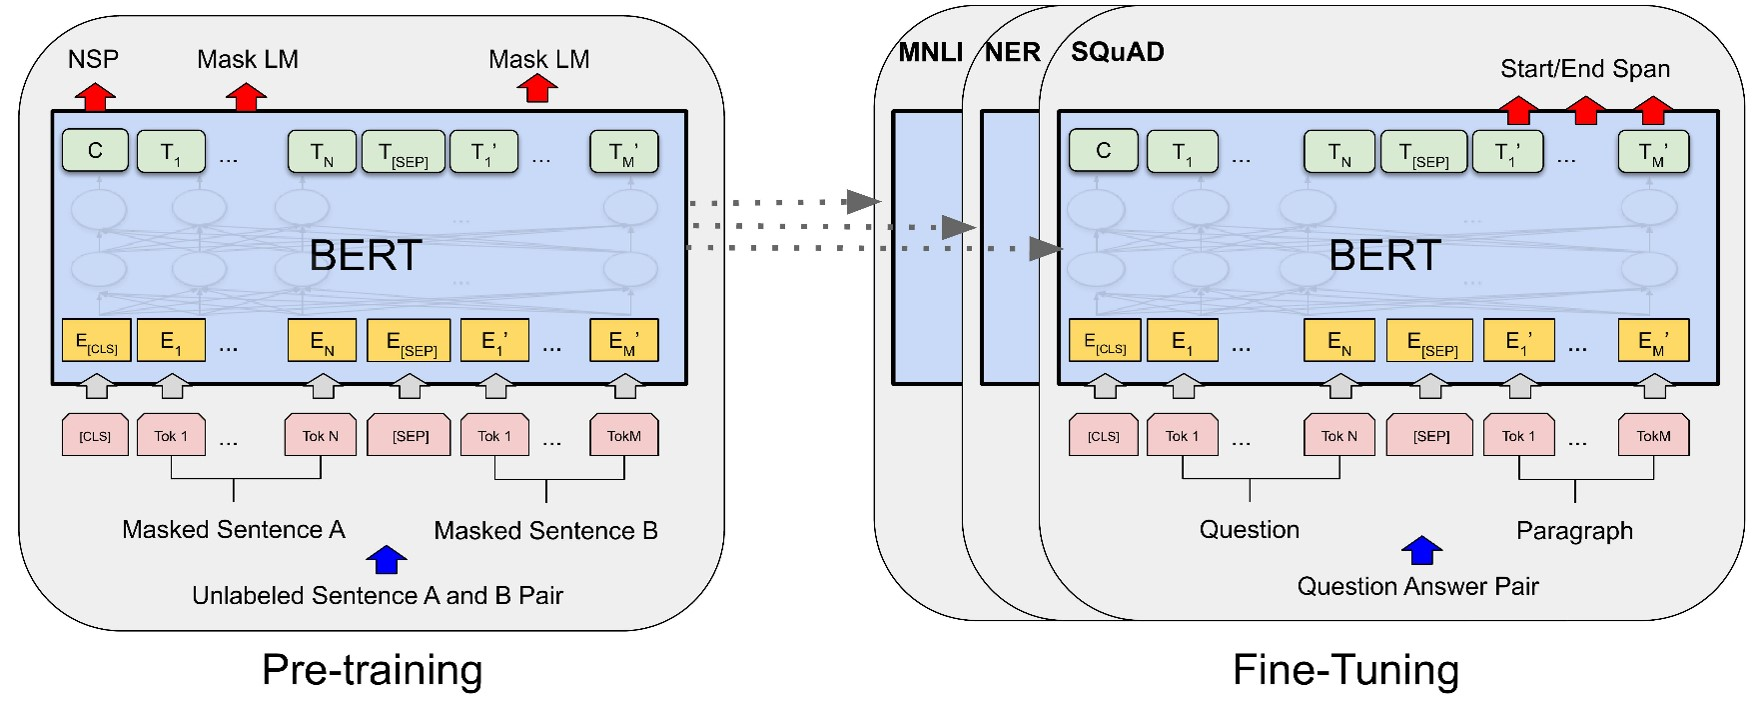
\includegraphics{img/BERT.jpg}}
\caption{Mô hình BERT\cite{devlin-etal-2019-bert}}
\label{fig:my_label}
\end{figure}
BERT được tiền huấn luyện (pretraining) với bộ ngữ liệu \textit{BookCorpus} (800 triệu từ) và \textit{Wikipedia English} (2500 triệu từ) với các pretraining task Masked Language Modeling (MLM) và Next Sentence Prediction (NSP), sau đó tinh chỉnh (finetune) lại cho từng task khác nhau. Sau khi BERT được công bố, nhiều mô hình cải tiến của BERT cũng được giới thiệu dựa trên kiến trúc của BERT, trong đó có thể kể đến
\begin{itemize}
\item \textbf{RoBERTa} (\textbf{R}obustly \textbf{o}ptimized \textbf{BERT} Pretraining \textbf{a}pproach)\cite{DBLP:journals/corr/abs-1907-11692}: sử dụng dynamic masking so với sử dụng static masking trong kiến trúc gốc; huấn luyện trên nhiều ngữ liệu hơn.
\item \textbf{DistilBERT}\cite{DBLP:journals/corr/abs-1910-01108}: mô hình nhỏ, nhanh, tốn ít chi phí huấn luyện hơn mô hình BERT gốc: có ít hơn 40\% parameters, chạy nhanh hơn 60\% nhưng hiệu quả bằng 95\% so với mô hình gốc.
\end{itemize}

\subsection{PhoBERT}
Dựa trên mô hình BERT, nhóm nghiên cứu từ VinAI đã công bố PhoBERT\cite{phobert}, được giới thiệu là mô hình ngôn ngữ đơn ngữ dành cho tiếng Việt có quy mô lớn đầu tiên. PhoBERT sử dụng quá trình pretraining của RoBERTa để tăng hiệu quả cho mô hình. Kiến trúc của PhoBERT vẫn giữ nguyên so với BERT:
\begin{itemize}
\item \textbf{PhoBERT\textsubscript{base}}: 12 encoder layers, 768 hidden units, 12 attention heads, 135 triệu parameters.
\item \textbf{PhoBERT\textsubscript{large}}: 24 encoder layers, 1024 hidden units, 16 attention heads và 370 triệu parameters.
\end{itemize}
PhoBERT được pretrain với bộ ngữ liệu \textit{Wikipedia Tiếng Việt} và bộ ngữ liệu tin tức tiếng Việt \textit{Binhvq News Corpus}.

\subsection{ViHealthBERT}
Mô hình ViHealthBERT sử dụng kiến trúc của BERT (12 encoder layer, 768 hidden units, 12 attention heads) với bộ trọng số huấn luyện của PhoBERT. Việc huấn luyện ViHealthBERT chia làm 2 giai đoạn:
\begin{itemize}
\item \textbf{Giai đoạn pretraining}: Huấn luyện trên các bộ ngữ liệu \textit{Text Mining Corpus} và \textit{OSCAR} : Masked Language Modeling (MLM), Capitalized Prediction (CP) và Next Sentence Prediction (NSP).
\item \textbf{Giai đoạn finetuning}: Finetuning trên các bộ ngữ liệu \textit{PhoNER\_COVID-19, VimQ, arcDrid} và \textit{FAQ Summarization}: Named-Entity Recognition (NER), Acronym Disambiguation và FAQ Summarization
\end{itemize}

\begin{figure}
\begin{center}
\resizebox{\textwidth}{!}{
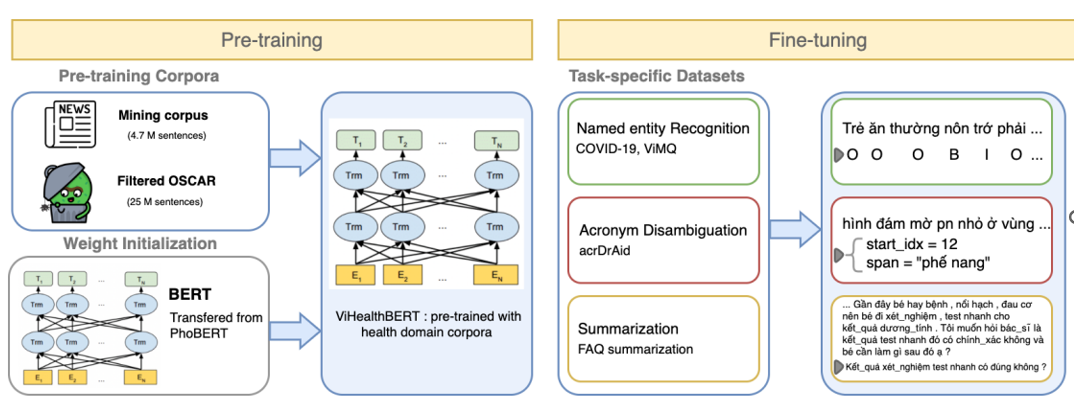
\includegraphics{img/ViHealthBERT.png}
}
\caption{Tổng quan về quá trình pretraining và finetuning trong ViHealthBERT\cite{minh-EtAl:2022:LREC}}
\end{center}
\end{figure}